\section{Numerical simulations}\label{Section5}

In this section, we will present several examples in which we solve our optimal control problem through the direct method and the non-linear constrained optimization tool \texttt{CasADi} \cite{Andersson2019}.
%
\subsection{Smooth approximation of piece-wise linear penalization}

With the final aim of using an optimization software to solve our optimal control problem, we will approximate our piece-wise linear penalization with the help of the Heaviside function $h:\mathbb{R} \rightarrow \mathbb{R}$ and its smooth approximation defined as follows: 
\begin{gather}
    h(x) = \begin{cases}
        1 & \text{ if } x \geq 0 \\
        0 & \text{ if } x < 0
    \end{cases}    
    \hspace{2em} 
    \begin{cases}
        h^\eta(x) = (1 + \tanh(\eta x))/2   \\
        \eta \rightarrow \infty
    \end{cases}
\end{gather}
Using $h$, we can define the (smooth) function $\Pi_{a,b}^\eta:\mathbb{R} \rightarrow \mathbb{R}$ as:
\begin{align*}
    \Pi_{[a,b]}^\eta(x) &= - 1 + h^\eta(x-a) + h^\eta(-x+b) 
    \\
    &= \frac{\tanh[\eta( x -a)] + \tanh[\eta (b-x)]}{2}.
\end{align*}
In this way, we can define the smooth version of \eqref{PLP}:
\begin{gather}
    \mathcal{L}^\eta(u) = \sum_{k = 1}^{N_u-1} \big[ (u_{k+1}+u_{k}) (u-u_k) + u_k^2 \big] \Pi^\eta_{[u_k,u_{k+1}]}(u)
\end{gather}
So that, when $\eta \rightarrow \infty$, then $\mathcal{L}^\eta \rightarrow \mathcal{L}$. 

\subsection{Direct method  for  OCP-SHE}

To solve the optimal control problem (\ref{pb:OCP_penalizado}), we use a direct method. 
%
If we consider a partition $\mathcal{P} = \{\tau_0,\tau_1,\dots,\tau_{T}\}$ of interval $[0,T]$ , we can represent a function $\{ u(\tau) \ | \ \tau \in [0,T]\}$ as a vector $\bm{u} \in \mathbb{R}^{T}$ where component $u_t = u(\tau_t)$.  
%
Then the optimal control problem (\ref{pb:OCP1}) can be written as optimization problem with variable $\bm{u} \in \mathbb{R}^{T}$. This problem is a nonlinear programming, for this we use CasADi software to solve. 
%
Hence, given a partition of the interval $[0,\pi)$, we can formulate the problem \ref{pb:OCP_penalizado} as the following one in discrete time
\newline

\begin{problem}[Numerical OCP]\label{pb:numOCP2}
Given two sets of odd numbers $\mathcal{E}_a$ and $\mathcal{E}_b$ with cardinalities $|\mathcal{E}_a| = N_a$ and $|\mathcal{E}_b| = N_b$ respectively, given the target vectors $\bm{a}_T  \in \mathbb{R}^{N_a}$, so that $\bm{x}_0 = [\bm{a}_T,\bm{b}_T]^T$ and $\bm{b}_T \in \mathbb{R}^{N_b}$ and a partition $\mathcal{P}_\tau = \{\tau_0,\tau_1,\dots,\tau_{T}\}$ of the interval $[0,\pi)$, we search a vector $\bm{u} \in \mathbb{R}^{T}$ that minimizes the following function:
\begin{gather}
        \min_{\bm{u} \in \mathbb{R}^{T} } 
        \Bigg[ 
        || \bm{x}^{T}||^2
        + \epsilon  
        \sum_{t=0}^{T-1} 
            \bigg[ \frac{\mathcal{L}^\eta(u_{t}) + \mathcal{L}^\eta(u_{t+1})}{2}\Delta\tau_t \bigg]  \Bigg]  \\
        \notag \text{suject to: } \\
        \forall \tau \in \mathcal{P} \begin{cases}
            \bm{x}^{t+1} = \bm{x}^{t} - (2/\pi)\Delta \tau_t \bm{\mathcal{D}}(\tau_t)u_t \\
            \bm{x}^0 = \bm{x}_0
        \end{cases} 
\end{gather}
\end{problem}

\subsection{Examples}

Todos los ejemplos que presentaremos a continuación tendrán en conmún los siguientes parámetros $\epsilon = 10^{-5}$, $\eta = 10^{-5}$ y una partición $\mathcal{P}_t = \{0.0 , 0.1, 0.2 ,\dots,\pi\}$.

%%%%%%%%%%%%%%%%%%%%%%%%%%%%%%%%%%%%%%%%%
%%%%%%%%%%%%%%%%%%%%%%%%%%%%%%%%%%%%%%%%%

\vspace{1em}
\begin{simulation}[Bang-Bang]\label{simu1}
Consideremos el Problema \ref{pb:numOCP2} con los siguientes parámetros $\mathcal{E}_a = \{1,5,7\}$ y  $\mathcal{E}_b = \{1,5,7\}$ y el control admisible en $\mathcal{U} = \{-1,1\}$. Además los vectores objetivos son: $\bm{a}_T = (i_d,0)^T$ y $\bm{b}_T = (i_d,0)^T$ para todo $i_d \in [-1,1]$. 

\begin{figure}[ht!]
    \hspace{0.05em}
    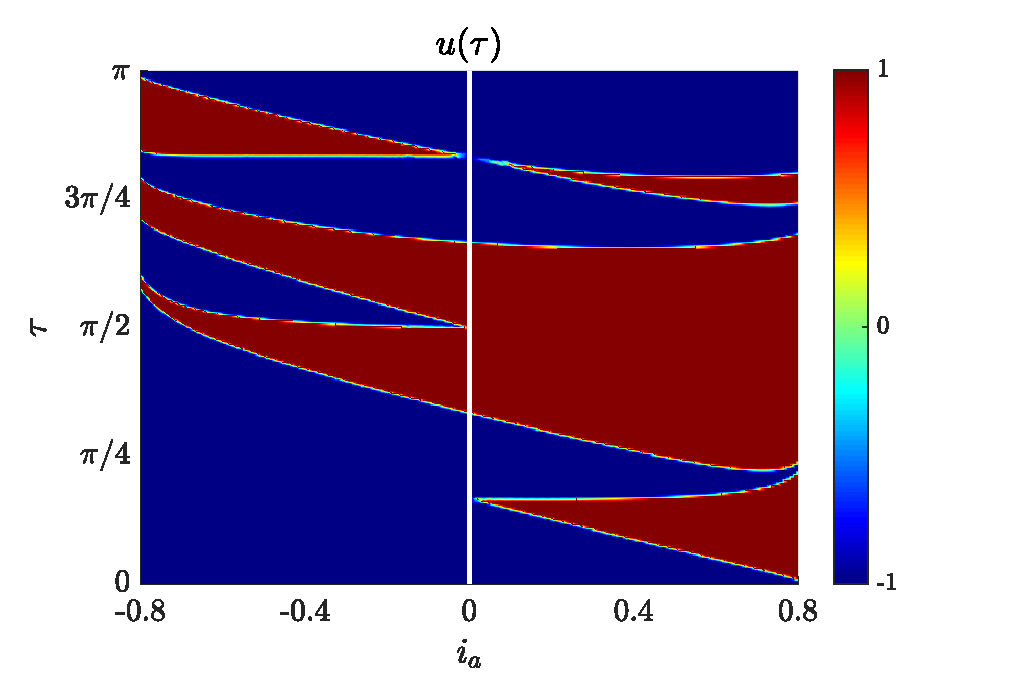
\includegraphics[scale=0.565]{img/fig05.eps}
    \caption{Results of simulation of Simulation \ref{simu1}.}
\end{figure} 
\end{simulation}
%%%%%%%%%%%%%%%%%%%%%%%%%%%%%%%%%%%%%%%%%
%%%%%%%%%%%%%%%%%%%%%%%%%%%%%%%%%%%%%%%%%

\vspace{1em}
\begin{simulation}[Bang-off-Bang]\label{simu2}

Consideremos el Problema \ref{pb:numOCP2} con los siguientes parámetros $\mathcal{E}_a = \{1,5\}$ y  $\mathcal{E}_b = \{1,5\}$ y el control admisible en $\mathcal{U} = \{-1,0,1\}$. Además los vectores objetivos son: $\bm{a}_T = (1/2,0)^T$ y $\bm{b}_T = (1/2,0)^T$  para todo $i_d \in [-1,1]$.  
\end{simulation}

\begin{figure}[ht!]
    \hspace{0.05em}
    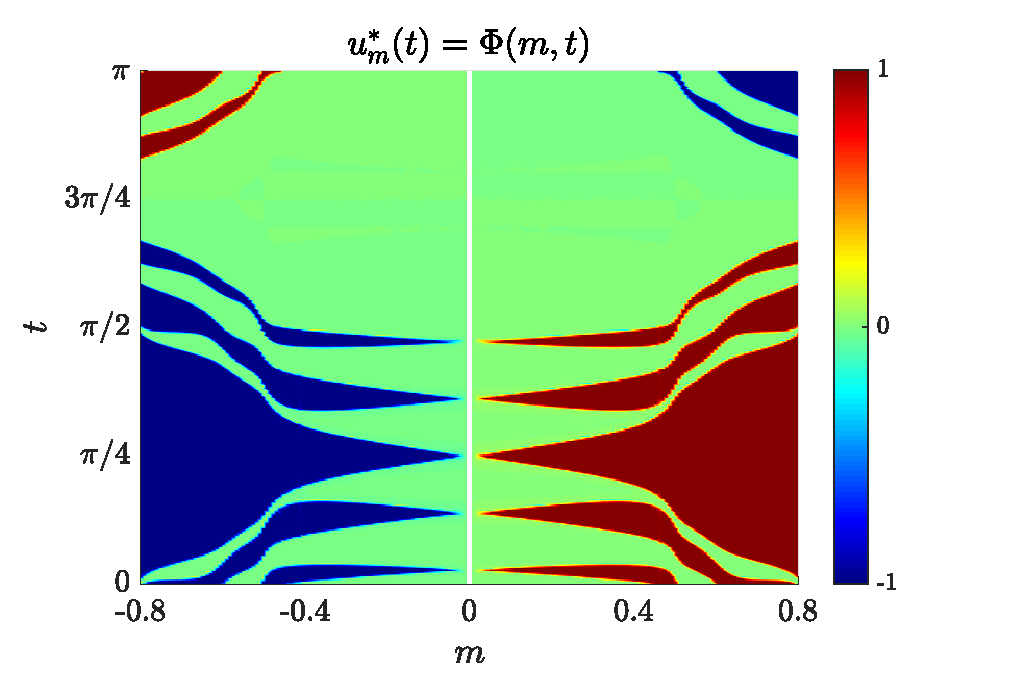
\includegraphics[scale=0.565]{img/fig06.eps}
    \caption{Results of simulation of Simulation \ref{simu2}.}
\end{figure} 

%%%%%%%%%%%%%%%%%%%%%%%%%%%%%%%%%%%%%%%%%
%%%%%%%%%%%%%%%%%%%%%%%%%%%%%%%%%%%%%%%%%
\vspace{1em}
\begin{simulation}[Multi-Nivel]\label{simu3}

Consideremos el Problema \ref{pb:numOCP2} con los siguientes parámetros $\mathcal{E}_a = \{1,5\}$ y  $\mathcal{E}_b = \{1,5\}$ y el control admisible en $\mathcal{U} = \{-1,-1/2,0,1/2,1\}$. Además los vectores objetivos son: $\bm{a}_T = (1/2,0,0)^T$ y $\bm{b}_T = (1/2,0,0)^T$  para todo $i_d \in [-1,1]$.  
\end{simulation}

\begin{figure}[ht!]
    \hspace{0.05em}
    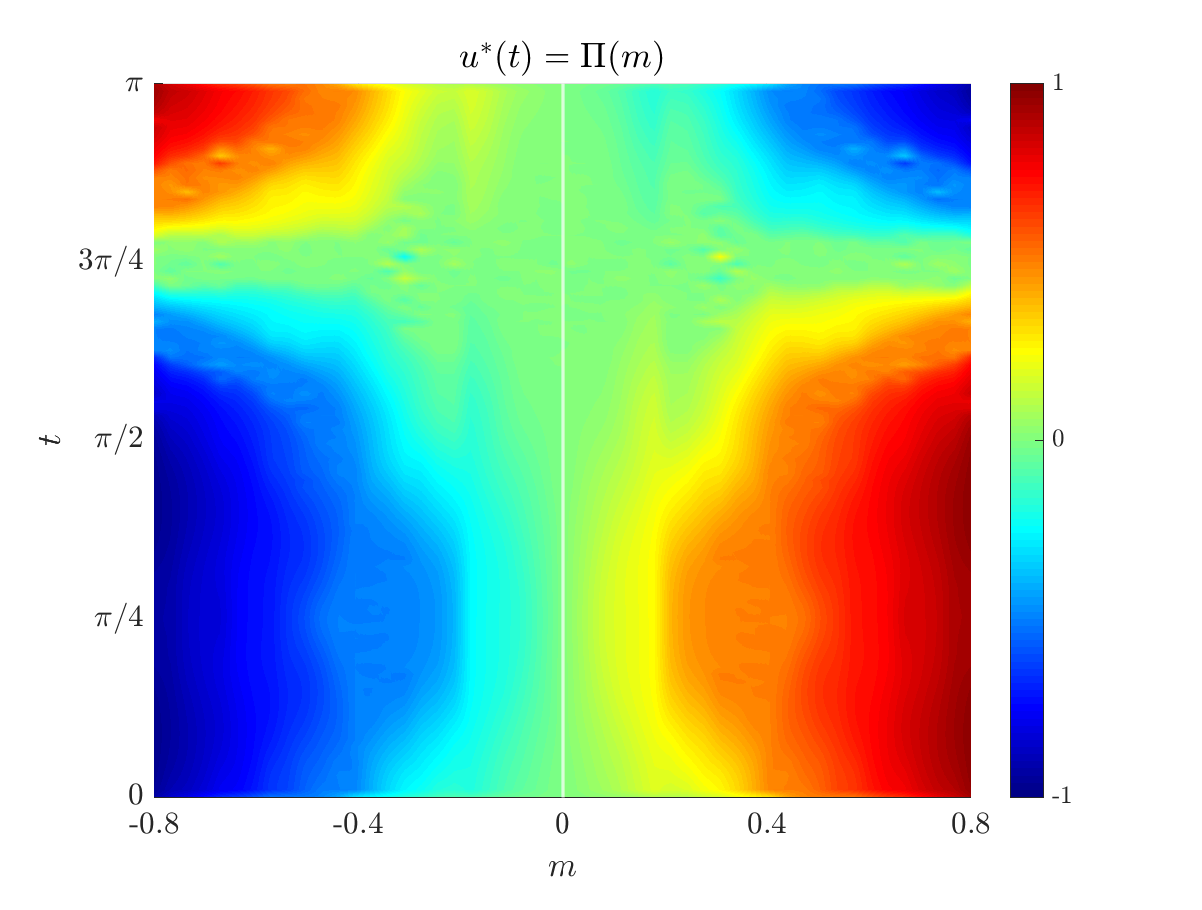
\includegraphics[scale=0.565]{img/fig07.eps}
    \caption{Results of simulation of Simulation \ref{simu3}.}
\end{figure} 
 